\documentclass{article}
\usepackage{graphicx}
\title{Lane change decision on highways, literature review}
\date{2024-09}
\author{Bedirhan Sen}
\begin{document}
  \pagenumbering{roman}
  \maketitle
  \newpage
  
  \section{Problem Description}
  \begin{itemize}
\item Mandatory lane change: Mandatory lane changes de-
fine the situations where drivers must perform a lane
change due to strict road rules and situations, such as
lane endings or lane blockages
\item Discretionary lane change: Discretionary lane
changes are performed by drivers when the observa-
tion indicates that, there is another lane with better
driving conditions for the host vehicle. 
\item Anticipatory Lane change: Finally, an-
ticipatory lane changes are performed to improve road conditions for other road actors, such as allowing a faster vehicle to pass .
\end{itemize}

Aim to determine when and how to execute a lane change maneouver. Under efficiency, safety and comfort criteria. 

3 categories of approaches to solve this problem
\begin{itemize}
\item Microscopic traffic models and decision trees
\item Markov decision process
\item Reinforcement learning. 
\end{itemize} 

task expected
from a decision-making module is to increase safety
and comfort while maintaining the desired speed.

  \section{Approaches From Literuature}
  
  \subsection{Automated Lane Change Decision Making in Highway using a Hybrid
Approach Caldıran et al}
\subsubsection{literature review}
Gipps(1986) introduced a decision-making model
that covers various urban driving situations. . Driver’s behavior is governed by two
basic considerations: maintaining the desired speed
and being in the correct lane for an intended turn-
ing maneuver.
Ahmed (1999) proposed lane change
decision-making models based on utility functions to
model microscopic highway traffic scenarios. The probability of
lane change was calculated based on the output of a
softmax function and the decisions of the drivers to
make lane changes were modeled using a decision
tree. 
Ardelt
et al. (2012) integrated the ideas from Ahmed (1999)
and Toledo (2003), and implemented a decision tree-
based framework based on utilities of adjacent lanes,
on an actual car. In the first phase, utilities of the
lanes are computed with a decision tree mechanism.
If the utilities indicate that a lane-change maneuver is
profitable, the feasibility of this lane change is then
controlled. If the lane change maneuver is not fea-
sible, a lane change gap approach protocol, whose
details were not provided, is activated.
Nilsson et al. (2016) computed three
types of utilities of adjacent lanes and assessed the
quality of gaps for a lane change.
A drawback of these utility-based methods is their
limited capacity regarding the incorporation of the
other traffic participants actions and their possible ef-
fects on the decisions.
n this regard, the Markov
Decision Process (MDP) and Partially Observable
Markov Decision Processes (PO-MDP) offer princi-
pled solutions to modeling and decision-making pro-
cesses. However, the implementation of MDPs or PO-
MDPs poses practical problems due to their computa-
tional complexity for real-time bound systems such as
autonomous cars. 
For example, Brechtel (2015) outlines highway
driving scenarios as a generic Markov Decision Pro-
cess with continuous states and action spaces based
on the dynamics and inputs of a car.
\subsubsection{Method}
We discretize the time from past the future and calculate
the utilities of lanes that belong to specific time inter-
vals. We created a utility table to keep utility values
from past to future, and we update the table at each
time step with the incoming utilities.

For future state prediction,
we use linear future state estimator functions that cal-
culate possible future velocities and positions of dy-
namic objects. 

Utility functions: 
\begin{itemize}
\item Longitudinal Velocity: The longitudinal velocity util-
ity represents the difference between the desired ve-
locity of ego and the actual velocity of ego 
\item Average Time Gap: The average time gap of a lane
represents the average of the time gaps between ve-
hicles in the corresponding lane. For the calculation,
the time gaps between longitudinally adjacent cars are
calculated and the average of these time gaps are used
as a utility factor.
\item Average Longitudinal/Lateral Velocity: These factors
denotes the average longitudinal and lateral velocities
in a specific lane. Based on the desired velocity of
ego, these factors can be used as hints to determine
which lane to keep.
\item Relative Leader Velocity: This factor denotes the
highest relative velocities in each lane. Even though it
is similar to the other velocity-related factors, know-
ing the fastest objects in lanes may help the driver
with the decision of keeping the current lane or not.
\item Presence of Heavy Vehicles: Presence of heavy ve-
hicles is an indicator of the inconvenient of a lane.
Lanes with heavy vehicles tend to be flowing slower
\item Required Number of Lane Changes: Required num-
ber of lane changes to reach a lane is an impor-
tant factor regarding driving safety and comfort. We
should avoid targeting far lanes as much as possible
and choose adjacent lanes to be sure about safety and
comfort
\item Presence of Tailgating: Tailgating is an undesirable
situation that can easily cause accidents. If a behind
vehicle is driving too closely, especially in the left-
most lane, the ego vehicle should make a lane change
to allow the vehicle to pass
\item Left/Right Most Lane Check: In highway, keeping the
left-most lane and right-most lane for a long time is
generally inhibited. Thus, keeping these lanes for de-
creases the utility of that lane over time.

\end{itemize}
For the overall utility calculation, we follow the
formulation in Ardelt et al. (2012). For each discrete
timestamp, we calculate the utilities of a lane from
past to future and get an overall utility value. Even
though past utilities are useful for a better assessment
of a traffic situation, they can imply wrong predictions
and slow down the utility process. 

\textbf{At first they do not think about where are the gaps and is it okay to do a lane change
they just asses the lane as a complete thing. Then there is a module to do a gap selection. }
When a lane change decision is made, our gap se-
lection algorithm searches for inter-vehicular gaps
that comply with certain safety and comfort crite-
ria. To find the best gap, the decision-making mod-
ule requires the kinematic information of the vehicles
around the ego vehicle for the whole 360◦ from the
environment perception modules.
The sensor fusion module, which is the core com-
ponent of the environment perception modules, uses
Kalman Filters to track the surrounding vehicles and
hence assumes a normal distribution for the uncer-
tainty in the estimated states of these vehicles.
Our gap selection algorithm considers both the estimated
kinematic states and their uncertainties for a feasi-
ble lane change as in Ardelt et al. (2012), i.e., the
rear/front bumper of a lead/follow vehicle is consid-
ered to be 3 standard deviations away from its es-
timated mean.

Furthermore, we estimate the future positions of
the surrounding vehicles using a constant acceleration
model to predict the future states of the inter-vehicular
gaps. Therefore, we can anticipate feasible but un-
reachable gaps to be reachable in a certain time hori-
zon and plan accordingly.
Nevertheless, gaps that are expected to be reach-
able in the future are not guaranteed to be reachable
or feasible in the expected time horizon (see Fig. 2a
and 2b). Therefore, gaps that are temporally closer to
the current time frame are more desirable.

Moreover,
aligning with a feasible gap might require a deviation
from the desired velocity, thus rendering the gap to
be less desirable. These criteria lead to another multi-
criteria selection problem among gaps. Similar to the
lane utility functions, we defined the following crite-
ria:
• Uto : Time for the gap opening
• Udur : Duration of the gap feasibility
• Utr : Time to reach the gap
• Uddv : Difference to desired velocity,

%\begin{figure}
 % \includegraphics[width=\linewidth]{fig1.png}
  %\caption{approach from paper 1.}
  %\label{fig:Gui}
%\end{figure}


  \subsection{Design of a utility-based lane change decision making algorithm and a
motion planning for energy-efficient highway driving
Sahar Zeinali}
  
  \subsubsection{literature review}
\subsubsection{Method}
The overall process of lane change can be divided into two steps,
including decision making, and planning and control. In the first step,
the desirability of the maneuver is checked via a decision making
algorithm. In the case of a desirable maneuver, its feasibility is checked
by an MPC-based trajectory planning. If the maneuver is feasible, a
lateral controller finds appropriate control inputs to execute the lane
change.
%\begin{figure}
 % \includegraphics[width=\linewidth]{fig2.png}
 % \caption{approach from paper 2.}
 % \label{fig:Gui}
%\end{figure}
%
The desirability of a lane change maneuver is checked via a decision
making algorithm, which is based on a utility function. This function
considers different aspects of the maneuver Li et al. (2020) and Nilsson
et al. (2016), such as:
1. Average travel time in lane ,
2. Remaining travel time in lane ,
3. Energy consumption in lane ,
4. Traffic rules.

\begin{itemize}
\item Average travel time Ulv
This variable shows the deviation of the average travel time of the
lane from the average travel time as expected from the desired velocity
vdes, set by the driver. It is defined as

where vdes and vl are the desired longitudinal velocity for the EV and
the average longitudinal velocity of the lanes l = c or l = t, respectively.
Also, gama > 0 is a parameter to avoid division by zero and dmax is the
maximum travel distance, defined as
dmax = Bvdes, (2)
where B is a positive constant. 
The average velocity of a lane is
calculated by taking an average of the velocities of the leading and
trailing vehicles in the lane.

\item 
Remaining travel time Uld
This parameter shows the time duration that the EV can stay in the
current lane l and is defined as
Uld = min(dmax, dend)/vdes 
where dend is the distance to the end point of the lane l
\item Energy consumption Ule
This variable shows the desirability of the lane change maneuver
from an energy efficiency point of view. In other words, by incorporat-
ing this variable, the lane with an average velocity closer to the optimal
operating point of the energy map is selected.
\item Traffic rules Ulr
In order to incorporate the rule of driving in the rightmost lane as
much as possible, the following utility function is considered: Ulr = -L
where L is the number of lanes to the right-hand side of the lane l.

A lane change maneuver is desirable if the utility function of the
target lane is higher than that of the current lane. In other words, if
Ut > (1 + e)Uc , where Uc and Ut are the total utility functions of the
current and target lane, respectively, and e is a positive parameter.
If a lane change is desirable, then in the next step, MPC as the
longitudinal planner, tries to find an appropriate engine or brake torque
to position the EV in the gap between the leading and trailing vehicles
in the target lane. For this purpose, the longitudinal dynamical model is
discussed in the next section, and then the energy-efficient MPC design
is presented in Section 4

\textbf{The motion of the TVs during the prediction horizon is predicted
by a constant velocity assumption.}

\end{itemize}
Lateral Trajectory planner: Utilizing a sigmoid function is another way to
design the trajectory. This function has beneficial mathematical charac-
teristics, such as continuity, differentiability, and a simple closed-form
expression. Furthermore, this function allows us to consider the dy-
namic and geometric constraints of the system, which is the most
important advantage
  \subsection{Lane Change Decision-making through Deep
Reinforcement Learning with Rule-based
Constraints Wang et al}
  	
  	\subsection{DQN deep q network}
  	
    \subsubsection{literature review}
    Wolf et al. [16] presented a method
for teaching an agent to drive a car in a simulation environment
by using DQN. The input of the network was the front-facing
camera image with a shape of 48×27, and the action space, i.e.
the network output, was discrete—5 actions were defined and
each corresponding to a different steering angle. The reward
function depended on the distance from the lane center and
some relative items (such as the error of the angle between the
vehicle and the center line). Hoel et al. [17] also used DQN
to deal with the problem of vehicle speed and lane change
decision-making in a simulation environment. Different from
previous work mentioned above, the Q-network input in [17]
was defined as a one-dimensional vector of the relative po-
sition, speed, and lane of surrounding vehicles, rather than
front-facing images. Two different agents were defined with
the discrete action space. The first agent considered only the
lateral lane change control, while the second considered both
the lane change and speed control. The result showed that the
second agent outperforms the former when CNNs were both
utilized. However, how to guarantee the decisions’ safety of
the learning-based method should be further considered.

\subsubsection{Method}
The
task of the decision-making module is to make an appropriate
driving decision according to the sensor information from the
perception module, and then plan a drivable path to the control
module
\textbf{Nevertheless, how to make a reliable decision is still a problem
for the rule-based methods owing to their poor ability to
generalize to unknown situations [11]}

\begin{figure}
 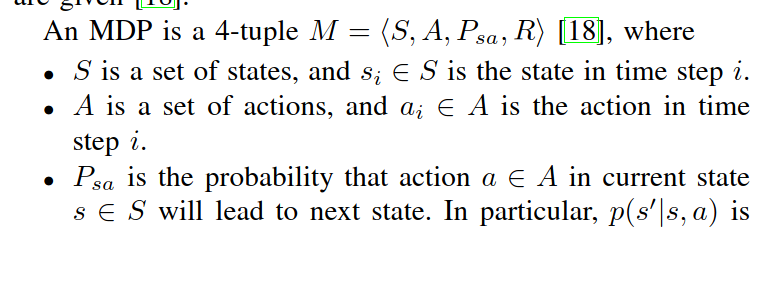
\includegraphics[width=\linewidth]{fig3.png}
 \caption{approach from paper 3.}
 \label{fig:Gui}
\end{figure}



  \subsection{Rule-Based Safety-Critical Control Design using Control Barrier
Functions with Application to Autonomous Lane Change}
    \subsubsection{literature review}
    ccording to
statistics provided by US National Highway Traffic Safety
Administration (NHTSA) in [1], about 9 percent of all vehicle
crashes involved lane change maneuvers. B. Sen, J. D. Smith, W. G. Najm et al., “Analysis of lane change
crashes,” United States. National Highway Traffic Safety Administra-
tion, Tech. Rep., 2003
\subsubsection{Method}
  \subsection{Integrated driving behavior modeling Toledo}
    \subsubsection{literature review}
\subsubsection{Method}
  
  \subsection{implementation from github}
  https://medium.com/@madhusudhan.d/path-planning-for-self-driving-cars-in-a-virtual-highway-fb266ba6713b
  The goal of the project to make a ego car drive around a virtual highway in dense traffic by adhering to following constraints for minimum 4.32 Miles.

    No collision at any time with other vehicles
    Maximum speed of 50 MPH (~ 80 KMH)
    Maximum acceleration of 10 m/s²
    Maximum jerk of 10 m/s³
    Vehicle cannot be in between lanes for more than 3 seconds
    Vehicle cannot go outside the 3 lanes of the highway
    Vehicle cannot drive on the wrong side of the highway
    
    planning code should output the trajectory of planned path to the term 3 simulator provided by Udacity, which will then visualize the ego behavior and output dynamic parameter like velocity, acceleration, jerk etc.
  
  \textbf{the simulator takes in position data in Cartesian coordinate system. However it can output position in Cartesian and Frenet Coordinate system. }
  
  \textbf{This module is heavily simplified in this project by using a Linear point model or constant velocity model for all the vehicles around the ego car. Given the duration for which the prediction is required, the new position of all the vehicles are calculated. }
  
  The basis of trajectory planning in this project is the map of highway given as text file highway map.csv. It is a cloud of points with each point described as both in cartesian and Frenet coordinate system. Format is as follows [X,Y,s,dx,dy].
  
  I think for path generation part  part of this map is isolated using the last 2 points in previous path and three more points selected over 90 m range. These five points are transformed from map coordinate system to vehicle coordinate system and interpolated using open source Spline function. For spline function they used https://kluge.in-chemnitz.de/opensource/spline/ The end result will be a spline starting from last position in previous path extending over 90 m along the track.
  
  They use a simulator which executes every point input in 20ms so the spacing between 2 points determines the vehicle speed. Then these points are transformed back the xy coordinate system. 
  
  They use 2 step system similar in the papers I looked for. 
  First lanes are ranked by cost functions and you choose the ideal lane to be in. 
  Then as a second step you choose the vacant area in that lane and make the change. 
  
  They used a fsm approach with 5 states,
      Keep Lane: 
    Prepare for Lane Change Left :
    Prepare for Lane Change Right: 
    Lane Change Left 
    Lane Change Right 
    
    Costs:
    \begin{itemize}
    \item goal\_lane\_cost : This function imposes higher cost on trajectories with vehicle in first or third lane and zero cost if the vehicle is in middle lane. Being in middle is efficient
    \item inefficiency\_cost : This function imposes higher cost on trajectories with intended and final lane that have traffic slower than the vehicle’s target speed. The function promotes lane change to maintain vehicle speed.
    \item lane\_change\_safety\_cost : This function imposes higher cost on trajectories that attempt lane change when speed difference between current lane and goal lane is less than 7 Kmph. This limits potential for accidents during lane change in heavy traffic
    lane\_chane\_safe\_dist\_cost : This function imposes higher cost on trajectories that attempt a lane change when front cars in both goal lane and current lane travel at same speed and distance ahead of ego car .This prevents waggling of ego cars
    \end{itemize}
    
  \subsection{Code decryption}
  generate predictions() of the class::Vehicle for the surrounding vehicle's state estimation with \textbf{constant velocity assumption} 
  
  The getXY helper function calculates the X and Y value given s and d in frenet coordinate system
  
  Behavior planning implementation is available in Vehicle.cpp . The function successor states() creates all these states. All the above states are coded in the functions keep lane trajectory(), prep lane change trajectory(), lane change trajectory(). These functions after checking for their respective conditions will call the function get kinematics() to calculate new position, velocity and acceleration. All these trajectories are then evaluated in test func() and trajectory with minimal cost is returned.
  
  All the cost functions are implemented in Cost.cpp. The function calculate\_cost() calculates weighted mean of the individual cost values.
  \end{document}